\chapter{客户参与} % Introduction chapter suppressed from the table of contents

\hypertarget{ux5e38ux89c1ux95eeux9898}{%
\subsection{常见问题}\label{ux5e38ux89c1ux95eeux9898}}

某软件离岸外包开发中心, 承接某政府医疗机构的IT系统维护工作
因为工作量变化很大,而且需要快速反应,
一直都是使用敏捷(Scrum)开发方式,每两周一个迭代
但因为甲方提需求的代表都是医护专业,缺乏软件开发和业务分析经验,
很多时候,每轮迭代提出的需求都很粗。
例如,护士办理病人住院:只发出一张表,
列举了各种人群病人的入院要求,步骤与条件。

乙方本来只使用敏捷开发的用户故事(User Story) 方式,
``护士办理病人住院''只算一个用户故事,难以判断:

\begin{itemize}
\tightlist
\item
  需求是否完整?
\item
  与其他功能的依赖关系。(例如,如可能有高度传染病,便必须先做某些化验,如果阳性便必须去隔离病房)
\item
  各种异常情景应怎样处理?
\end{itemize}

为了避免开发出来的功能不能满足需求,必须靠乙方开发团队先做好详细分析,但他们反而不太懂业务,导致只能从技术角度分析,未能全面挖掘业务特性。

\hypertarget{ux6539ux8fdbux65b9ux6848}{%
\subsubsection{改进方案}\label{ux6539ux8fdbux65b9ux6848}}

\begin{itemize}
\tightlist
\item
  使用功能点识别实体与行为

  \begin{itemize}
  \tightlist
  \item
    便能容易识别出需求中,那些地方甲方没有考虑例如,除了新增,是否也需要有查询和删除功能
  \end{itemize}
\item
  再利用用例(Use cases)
  与各种场景(scenarios)和对应系统页面原型图,与甲方代表讨论各种场景,系统应如何处理
\end{itemize}

\hypertarget{ux6539ux8fdbux6548ux679c}{%
\subsubsection{改进效果}\label{ux6539ux8fdbux6548ux679c}}

\begin{itemize}
\tightlist
\item
  挑了两个医疗相关的团队做试点,在开发前,用了这些方法预先与甲方充分讨论,三个月,6轮迭代后,UAT里的需求相关缺陷数平均降低43\%。
\end{itemize}

从以上案例看到,客户代表除了要参与,还要有具体措施做好需求,例如可利用功能点方法,用例与场景来挖掘与分析需求。

\hypertarget{ux8bc6ux522bux5229ux76caux76f8ux5173ux8005}{%
\subsection{识别利益相关者}\label{ux8bc6ux522bux5229ux76caux76f8ux5173ux8005}}

和杭州客户领导吃晚饭,领导就跟同桌的项目经理开玩笑说,``你们刚刚完成内部项目管理自动化工具,做调研的时候好像没有找过我?
其实,我是其中一位经常要使用这系统的管理者,下面项目的监控、申请都是经过我,但我发现这个系统很不合用,对收集我需要的项目信息没有作用。比如没办法处理一些批准信息。''\\
从上面对话,可以了解如果没有全面识别项目的利益相关者,可能会影响到项目的成败。例如,我接触一些有些具备开发经验的需求人员,但他们通常只注意功能需求的技术细节。

他们,“哪些是你的项目干系人?”很多人都会说,“甲方有协调员,要访谈哪些人都是由甲方协调员安排,我们听他安排。”所以为了避免未能识别所有干系人的风险,就要主动跟甲方一起策划。我们说沟通计划必须是甲乙方一起合作做出来,而且会牵涉甲乙方各个层次的人。

例如要听甲方出资人的需求,可能就要乙方的总经理出马,乙方的需求人员顶多可以跟甲方对口的项目组人员沟通。如何可以做好识别干系人,并制定沟通计划可详见附件。

\hypertarget{ux7528ux6237ux6545ux4e8bux5361}{%
\subsection{用户故事卡}\label{ux7528ux6237ux6545ux4e8bux5361}}

用户故事卡目的是让用户(业务)与开发沟通交流。

虽然Kent BECK先生强调用户故事卡片上的东西并非交流的全部,
也不应该包括太多细节。
但XP/Scrum的用户故事卡片未能全面包括需求的各元素,例如缺乏:

\begin{itemize}
\tightlist
\item
  来源: 每项需求都应可追溯到源头
\end{itemize}

\begin{itemize}
\tightlist
\item
  冲突:确保需求之间的一致性
\end{itemize}

\begin{itemize}
\tightlist
\item
  顾客满意度 / 顾客不满意度:用两个数比单纯用优先级能更全面反应客户声音
\end{itemize}

%\href{文件:9_用户故事1.png}{450px}


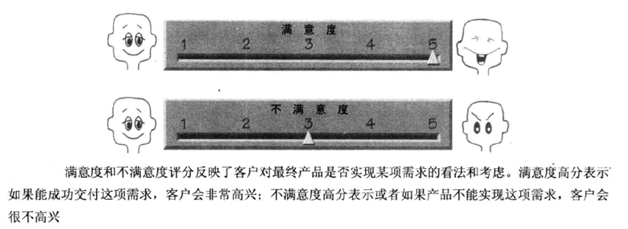
\includegraphics[width=10cm]{9_用户故事1.png}

\begin{description}
\tightlist
\item[]
(如想多了解为什么要这样分,请看附件里的``客户声音: Kano Diagram'')
\end{description}

卡片例子,可参考ROBERTSON夫妇的需求卡片模板:

%\href{文件:9_用户故事2.png}{500px}

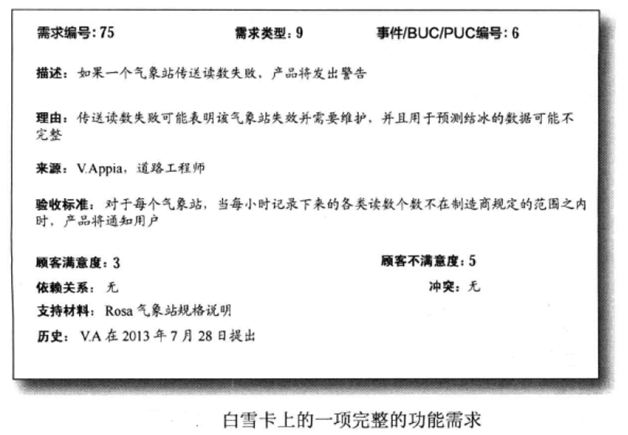
\includegraphics[width=10cm]{9_用户故事2.png}

也可以用于非功能需求:\\
%\href{文件:9_用户故事3.png}{500px}

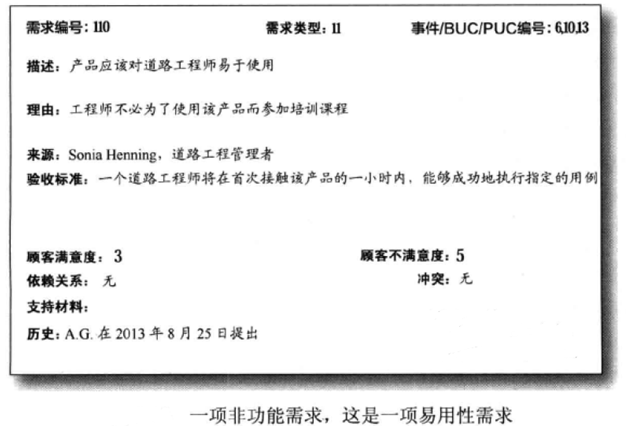
\includegraphics[width=10cm]{9_用户故事3.png}

\begin{itemize}
\tightlist
\item
  千万不要误以为卡上的所有信息都需要一次性与用户获取
\item
  挖掘需求永远是持续,并不断细化
\item
  卡片上增加了这些部分,可提醒我们不要忽略这些元素
\end{itemize}

\hypertarget{ux7528ux4f8bux4e0eux573aux666f}{%
\subsection{用例与场景}\label{ux7528ux4f8bux4e0eux573aux666f}}

用户故事针对 `做什么'与 `为什么' ("What", "Why"); 用例与各种场景
针对`如何做' ("How" ),所以它们之间是互补,没有冲突。

下面用大家都熟悉的简单系统 -- ``在核酸检查点做检查,并提交结果'' --
来举例说明,如果考虑不周全,也会导致需求相关问题。

%\url{文件:CI场景图.jpg}

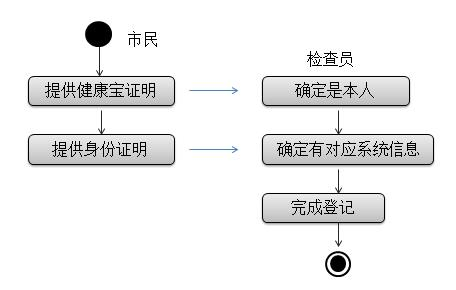
\includegraphics[width=10cm]{CI场景图.jpg}

\textbf{正常情况}:使用大陆身份证时,用读卡器获取实名身份信息,与系统记录对应,记录信息也齐全,包括手机电话号码。\\
\textbf{其他可选情况}:没有大陆身份证,其他证件,例如港澳通行证、国外护照。\\
\textbf{异常情况}:市民身份信息不能用读卡器自动获取,需要手工输入,但检察员输入信息错误。例如护照号码错误,手机号码为空,被删掉或者没输入。\\
如果问需求分析师、产品经理有什么异常场景;一般都会回应''没有``;部分回应一些最基本的异常,例如,``只有输入信息错误;报错;要求重新输入'',我便会以我的经验举例,说明必须要识别各种异常场景,才能算全面挖掘需求;识别正常场景是基本工,能识别各种异常场景才算做好。

\framebox{%
\begin{minipage}[t]{0.97\columnwidth}\raggedright
我每次在北京做免费核酸检测,因为非大陆身份证,检测员都要用手机手工输入我的信息:
姓名,港澳通行证号(因为系统已经有我的手机号,所以通常不需要再输入手机号),
只要我确认以上信息都输入正确,通常都没有问题。

后面不知道为什么原因? 不再用手机,改用笔记本电脑,配电子读卡器
阅读电子身份证,和电子扫描器读二维码。

检测员不再要手工输入我的信息, 靠我预先进系统填好所有信息,生成二维码,
只要检测员验证了我的二维码信息与系统信息对应,便可完成。

一般正常操作是没有问题的。

但我最近在某采集点检查完,之后第二天未能在我健康宝正确展示出核酸结果。(开头以为出现了``混管阳性'',但之后几次核酸结果又回复正常。)

我遇到的问题可能是因为那个采集点使用了笔记本电脑,信息先存在电脑,最后才批量上传到服务器。但因为非大陆身份证的情况,没有检查清楚信息是否都完备,例如,可能某些信息被检察员错误删掉了,但电脑没有报异常,最终批量上传时,服务器便无法识别我的检查记录。
以上只是我的猜测,估计永远都不会知道真正答案,但无论如何,如果当初系统分析时能全面识别所有场景,应可避免这类问题。\strut
\end{minipage}}

\framebox{%
\begin{minipage}[t]{0.97\columnwidth}\raggedright
如果使用银行交易系统概念,应可避免这类错误。比如我从自己账号转钱到另一个人的账号,中间会经过多家银行,我提交后,系统都会确保中间每一轮交易都已成功完成,并确认对方银行最终收到款,才算完成这个交易(通常前后经过几分钟)。中间任何环节出问题,都会撤回整个交易,能避免出现我那种不了了之的情况了。\strut
\end{minipage}}

如果信息有误或者不成功,导致最终无法提交上线,怎么处理?因总服务器本身或网络出问题无法连上,怎么处理?\\

如果要充分考虑各种异常情况,应仔细询问以下一系列问题:\\
%\href{文件:12_场景5.png}{550px}

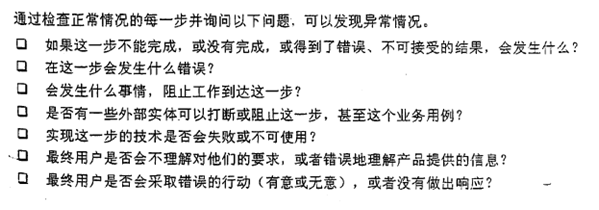
\includegraphics[width=10cm]{12_场景5.png}

另外一类情况,有几十人排队等待做核酸,原因是服务器出了问题,停机了,排队人非常不满。工作人员也很尴尬说已经想尽办法用手机、电脑,但是都没办法。如果提前想好这种场景,就可以在本地把相关信息记录下来,等个服务器恢复后一次性上传,就可以减少刚才的情况。\\

除了正常,也可以考虑一些\textbf{假设的场景},让干系人、客户可以更开放地考虑各种不同的情况,更创新。例如,是否可以考虑像超市付款一样,自主处理?当很多人排队的时候,就不会因为检察员一个人忙不过来,导致排长队。\\
例如,取登机牌也可以用机器,让乘客自主一组办理。其实做核酸也可以这样处理。\\
所以从以上案例看到用例+场景 不同于用户故事,可以弥补后者。Kent
BECK先生特别提倡用户故事,因为当时很多客户都觉得用例太细,太偏技术,不愿意写,甚至也不愿意读;但客户大多都愿意用自然语言
写用户故事,可以很容易触发客户与开发交流沟通。

但如果需求分析师只考虑现在业务流程的各种场景,开发人员开发系统,把所有的场景都覆盖好,是否便能成功?
不一定,请看以下例子:

\hypertarget{ux4e3eux4f8b}{%
\subsection{举例}\label{ux4e3eux4f8b}}

你们都有申请过护照吗?
比如我们护照更新,以前是要到柜台手工办理,如果我们把那个过程数字化,应该怎么做呢?

某国家的做法是本来的手工填写模板直接变成系统页面(每个输入与手工表格一一对应),申请人在系统里按本来模板填写并提交,上传个人新照片,也是经过系统,我有一次尝试用系统线上填电子表单申请,但因表单很繁琐,有很多护照原有信息都需要重新填写,光是填那表就花了我接近一个小时,最大问题还不是在我花时间填手工表,而是最后要上传照片,因为照片像素高的话就很大,需要很好的网络才可以传得上,如果照片像素小,便导致模糊不清,不能通过。最后,一个半小时后,我用尽所有方式都还是无法传上照片,我最终放弃了在线上提交申请,直接预约去在柜台做!\\
客户:有好方法解决这问题吗?\\
我:有,另外某国家的做法就很简单多了:\\
之前描述的整个过程只是把原有的手工步骤信息化,和原本的申请手续一样。但线上办理和在柜台现场办理不同,在现场你可以要求对方直接把照片给你,也可以要求对方提供老护照,但在线上办理,应很容易从系统里找到个人护照信息,所以很多本来在柜台要手工填写的老护照信息就不需要再填了。
客户:怎么可以简化整个过程?最困难应是照片的更新?
我:有些国家是这样做法,比如你申请续证,只需要填上老证件的基本信息,系统就立马能识别出本来的证件
你确实有那个`旧'证后,便可立马提交申请。跟在网上购物一样,你确认过内容没问题,就在网上付费,然后打印申请表并在表上亲手签字,然后附上几张符合规格的照片,邮寄到政府机关。他做好新证件以后再邮寄回你。或者你自己到他规定的地点领取也可以。
这样就能很简单地利用`低'科技解决方案,解决了刚才上传照片的困难。

从上面例子看到,我们应不仅是把那些本来手工的流程自动化,应该全局看要解决的问题本身,哪些过程自动化,哪些不应该自动化,(比如传照片)

甲方对怎么可以在线上做这个过程也没有概念,他只是知道,本来手工需要填表。
乙方也不知道,他只是做开发,也不知道有什么方面可以不用IT方式,而用其它方式更合理。
必须要一起探讨才可以有最好的解决方法。

所以作为业务分析师,你很可能要改变用户思考问题的方式,例如,利用业务过程模型,配合场景与页面原型,与利益相关者一起探索问题的本质。软件系统必须为拥有它的人提供最理想的价值,构建软件系统本身(例如,只是把现有流程自动化)不一定能解决客户业务问题。

\hypertarget{ux603bux7ed3}{%
\subsubsection{总结}\label{ux603bux7ed3}}

除了有客户参与团队,快速反馈,也要:

\begin{itemize}
\tightlist
\item
  全面识别所有利益相关者
\item
  利用功能点分析,了解范围,确保需求完整
\item
  利用用例与各类场景,全面了解各业务事件都可度量,可测试
\item
  利用需求卡片记录用户故事
  (因与干系人沟通,获取需求是持续逐步细化过程)
\end{itemize}

\hypertarget{ux9644ux4ef6}{%
\section{附件}\label{ux9644ux4ef6}}

\hypertarget{ux5229ux76caux76f8ux5173ux8005ux8ba1ux5212ux68c0ux67e5ux5355-stakeholders-plan-checklist}{%
\subsection{利益相关者计划检查单 (Stakeholders Plan
Checklist):}\label{ux5229ux76caux76f8ux5173ux8005ux8ba1ux5212ux68c0ux67e5ux5355-stakeholders-plan-checklist}}

{[}For each item, refer to notes for examples /
explanation{]}对于每个项目,参阅实例/解释\\
1/ List all potential stakeholders列出所有潜在的利益相关者\\
1a. What are the base Segments 类型 / 分组?\\
1b. Any sub-segments ?任何子段\\
2/ Assign F (Friendly), I (Ignore), U (Unfriendly) to them\\
给它们指定F(友善),I(忽略),U(不友好)\\
3/ What is important to them?\\
对他们来说什么是重要的?\\
4/ Learning objectives: 学习目标\\
For each stakeholder, what will we need to learn?\\
对于每一个利益相关者,我们需要学习什么?\\
5/ How ? 怎样沟通?\\
6/ When ? 时间安排?\\
7/ Sampling plan. 抽样计划 How to recruit 如何招募?\\
How to get commitment 获得承诺?\\

%\hypertarget{ux5907ux6ce8notes}{%
%\subsection{备注Notes}\label{ux5907ux6ce8notes}}

\hypertarget{ux6539ux8fdbux65b9ux6848}{%
\subsubsection{备注Notes}\label{ux6539ux8fdbux65b9ux6848}}

1/ Stakeholders 全面考虑各类利益相关者\\
%\href{文件:7_利益相关者1.png}{文件:7 利益相关者1.png}

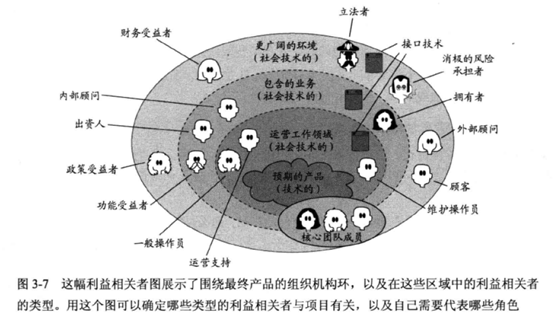
\includegraphics[width=10cm]{7_利益相关者1.png}

出资人 (Sponsor):出资人为产品的开发付钱\\
顾客
(Customer):顾客购买产品。必须对他们有足够的了解,理解他们认为什么有价值,所以会购买什么产品。\\
用户
(User):确定用户的目的是为了理解他们所做的工作,以及他们认为哪些改进有价值。\\
在开发消费产品、大市场软件时,应该考虑用一个``假想用户''。假想用户是一个虚拟用户,他是大多数用户的原型。\\
类型/分组的例子:\\
\textbf{未来笔记本电脑的潜在用户}:\\
大类:\\
\#商业人士 (Business)

\begin{enumerate}
\tightlist
\item
  媒体专业人士(Media Pro)
\item
  家庭用户(Home)
\end{enumerate}

细分:\\
\#主要用户(Lead User)

\begin{enumerate}
\tightlist
\item
  对产很有要求的(Demanding)
\item
  潜在用户(Potential)
\item
  对技术很有追求的 (Tech-Phobic)
\end{enumerate}

%\href{文件:CustomerMatrixScreenshot_2022-12-16_180326.jpg}{600px}

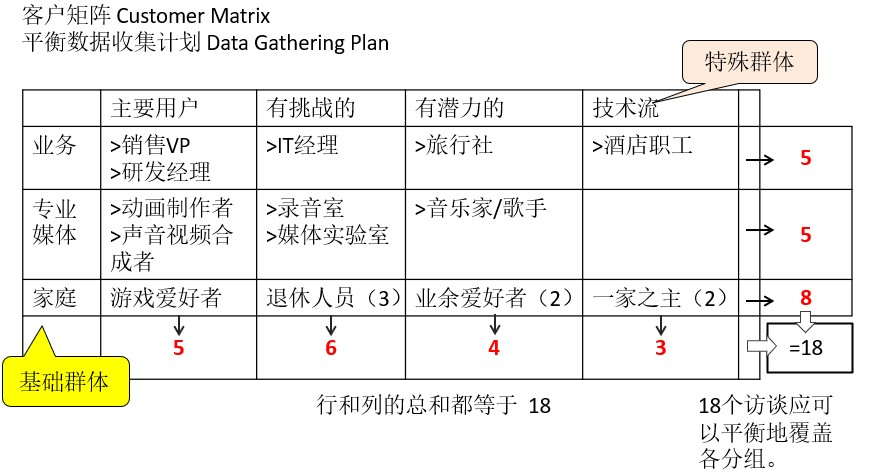
\includegraphics[width=10cm]{CustomerMatrixScreenshot_2022-12-16_180326.jpg}

2/ User inclusion strategy 包括哪些用户的策略\\
依据设计人员会怎么对应,把不同识别出来的利益相关者分成F、I、U\\
例:以针对笔记本电脑创新产品\\
F(Friendly)友好- 比如家庭用户、商业用户、媒体专员\\
I(Ignore)不考虑 - 比如忽视残疾人士\\
U(Unfriendly)不友好/消极的 - 比如黑客; 小孩(禁止他下载游戏、玩游戏)\\
3/ 他们的主要关注点------注重什么?

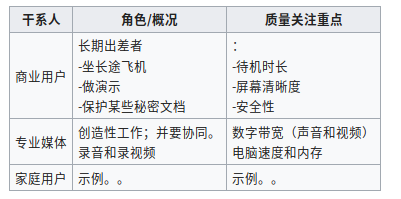
\includegraphics[width=10cm]{Screenshotfrom2022-12-2807-16-55.png}

有些在调研之前可能已知.......其他需要挖掘

\hypertarget{ux5ba2ux6237ux58f0ux97f3kano-diagram}{%
\subsection{客户声音:Kano
Diagram}\label{ux5ba2ux6237ux58f0ux97f3kano-diagram}}

可以用下图分析用户对需求优先级:

%\href{文件:IcKanoDiagramScreenshot_2022-12-17_120845.jpg}{600px}

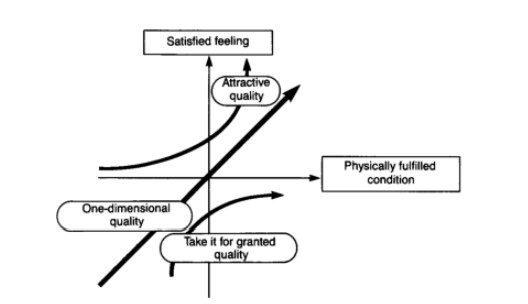
\includegraphics[width=10cm]{IcKanoDiagramScreenshot_2022-12-17_120845.jpg}

\begin{itemize}
\tightlist
\item
  解读上下两个箭头应怎样看:

  \begin{itemize}
  \tightlist
  \item
    下面的箭头代表(Take it for
    granted):如果缺乏,客户会很不满意;包括觉得是理所当然\\
  \end{itemize}
\end{itemize}

( 例如:满意度:中立 1 , 不满意度: 非常不满 5)

\begin{itemize}
\item
  \begin{itemize}
  \tightlist
  \item
    上面的箭头代表是加分项
    (Attractive),如果包括会非常满意,但如果缺乏不会觉得不满意\\
  \end{itemize}
\end{itemize}

( 例如:满意度:非常满意 5 , 不满意度: 中立 1)

所以用两个系数:满意 +
不满意,可以帮助判断某功能属于那类,哪一类的功能需求。

\hypertarget{references}{%
\section{References}\label{references}}

1. BECK, Kent . D. WEST: "User Stories in Agile Software Development" ,
Ch.13 of \emph{Scenarios, Stories, Use Cases: Through the Systerms
Development Life-Cycle}edited by F Alexander(2004)\\
2. COHN, Mike : ''User Stories Applied ''(2004)\\
3. MARTIN, Robert C.: \emph{Clean Agile - Back to Basics}\\
4. ROBERTSON, S. : ''Mastering the requirements process ''(2/e) (2006)\\



